% Created 2024-02-29 Thu 15:38
% Intended LaTeX compiler: pdflatex
\documentclass[11pt]{article}
\usepackage[utf8]{inputenc}
\usepackage[T1]{fontenc}
\usepackage{graphicx}
\usepackage{longtable}
\usepackage{wrapfig}
\usepackage{rotating}
\usepackage[normalem]{ulem}
\usepackage{amsmath}
\usepackage{amssymb}
\usepackage{capt-of}
\usepackage{hyperref}
\hypersetup{colorlinks=true, allcolors=blue} \usepackage{titlesec} \usepackage{geometry} \geometry{margin=1.2in} \usepackage{minted} \newcommand{\sectionbreak}{\clearpage} \usepackage{graphicx} \usepackage{changepage} \usepackage{inconsolata}
\author{Matthew}
\date{\today}
\title{}
\hypersetup{
 pdfauthor={Matthew},
 pdftitle={},
 pdfkeywords={},
 pdfsubject={},
 pdfcreator={Emacs 28.3 (Org mode 9.7)}, 
 pdflang={English}}
\begin{document}

\begin{LATEX}
\begin{titlepage}

  \centering
  {\Large\bfseries Big Data Assignment 1 \par}
  \vspace{0.5cm}

  {\large CRGMAT002 GRDDAN017 KFWJOR001 MRCGAB004 WHLJOS001\par}
  \vspace{0.5cm}

  {\large March 1, 2024\par}

  \vspace{2cm}
  
\includegraphics[width=0.4\textwidth]{mongo.png}
  
\includegraphics[width=0.4\textwidth]{uct.png}
\end{titlepage}
\tableofcontents
\end{LATEX}
\pagebreak
\section{Find or Create a Suitable Data Set}
\label{sec:org574278c}
\subsection{Data Set Explanation}
\label{sec:org9be7cf1}
Link to the dataset: \url{https://github.com/zygmuntz/goodbooks-10k}\\
\linebreak
The dataset includes data from an online book review platform (\url{https://goodreads.com/}). It includes information about the books, users, book tags, and book rating scores. The dataset initially contained multiple csv files. This dataset was chosen as its ideal for a MongoDB database due to its semi-structured nature and nested data, which is particularly useful for storing ratings and book tags. \\
\linebreak
\textbf{Dataset Content}:
\begin{itemize}
\item \textbf{books.csv}: Each entry represents a book with a unique \texttt{book\_id}. There are multiple data fields for a book:
\begin{itemize}
\item \textbf{\texttt{book\_id}, \texttt{goodreads\_book\_id}, \texttt{best\_book\_id}, \texttt{work\_id}}: Unique id’s representing a book, each with a different purpose. We only used \texttt{book\_id} and \texttt{goodreads\_book\_id} as they’re used to link books to user \texttt{ratings} and user \texttt{to\_read} lists.
\item \textbf{\texttt{ratings\_1}, \texttt{ratings\_2}, …}: Number of user ratings by rating value. eg. \texttt{ratings\_1} represents the number of 1 star ratings given to that book.
\item The rest of the fields are self explanatory but include info relating to authors, title, release date, and isbn number.
\end{itemize}
\item \textbf{ratings.csv}: Each entry is a \texttt{user\_id} to \texttt{book\_id} mapping with a rating.
\begin{itemize}
\item \textbf{\texttt{book\_tags.csv}}: Each entry is a \texttt{book\_id} to \texttt{tag\_id} mapping.
\item \textbf{\texttt{tags.csv}}: Each entry is a tag\textsubscript{id} to \texttt{tag\_name} mapping.
\item \textbf{\texttt{to\_read.csv}} : Each entry is a \texttt{user\_id} to \texttt{goodreads\_book\_id} mapping which represents a user adding a book to their \texttt{to\_read} list.
\end{itemize}
\end{itemize}
\subsection{Data Pre-Processing}
\label{sec:org27bc270}
The data was processed such that the data was represented in JSON format with evidence of nested objects so that we could demonstrate the capabilities of MongoDB.\\
\linebreak
Here is a quick outline on how we processed the data to create JSON files:\\
Libraries used: \texttt{Pandas}, \texttt{PyArrow}, \texttt{Faker}\\
\linebreak
\texttt{Pandas} was used to load the csv files into dataframes where we merged data and applied \texttt{group by} aggregate functions to obtain lists of data objects per a unique entry id. This was useful, for example, when we obtained a list of tags per \texttt{book\_id}.\\
\linebreak
\texttt{Faker} was used to generate random usernames for each id that were then written to \texttt{user\_data.csv}. The \texttt{dataframes} were then converted into JSON files.\\
\linebreak
All data pre-processing code is in the data-processing directory but the output JSON files are included in the final submission.
\section{Design a MongoDB Database}
\label{sec:org6d5b723}
Both Collection Schemas were designed by creating hand-made JSON example objects. Each of these objects shows what a document in the DB would look like. Underneath each JSON example, we have included a diagram which represents the example's nesting visually.
\subsection{Collection 1 - \texttt{books}}
\label{sec:org7061072}

\paragraph{JSON example} \small
\begin{minted}[]{js}
{
    "book_id": "98",
    "isbn": "1401359604",
    "isbn13": "9781401359610.0",
    "authors": [
        "Plum Sykes"
    ],
    "original_publication_year": 2004,
    "title": "Bergdorf Blondes",
    "language_code": "en-US",
    "average_rating": 3.26,
    "ratings_count": 23795,
    "total_ratings": {
        "ratings_1": 2020,
        "ratings_2": 4428,
        "ratings_3": 8669,
        "ratings_4": 6144,
        "ratings_5": 4561
    },
    "image_url": "https://s.gr-assets.com/assets/nophoto/book/111x148-bcc042a9c91a29c1d680899eff700a03.png",
    "tags": [
        {
            "tag_id": 11743,
            "tag_name": "fiction"
        },
        {
            "tag_id": 8717,
            "tag_name": "currently-reading"
        },
        {
            "tag_id": 8055,
            "tag_name": "contemporary"
        }
    ],
    "ratings": [
        {
            "user": {
                "user_id": 237,
                "user_name": "David Smith"
            },
            "rating": 1
        },
        {
            "user": {
                "user_id": 364,
                "user_name": "Christina Calderon"
            },
            "rating": 1
        },
        {
            "user": {
                "user_id": 399,
                "user_name": "Stephen Pugh"
            },
            "rating": 2
        }
    ]
}
\end{minted}

\newgeometry{margin=0in}
\begin{center}
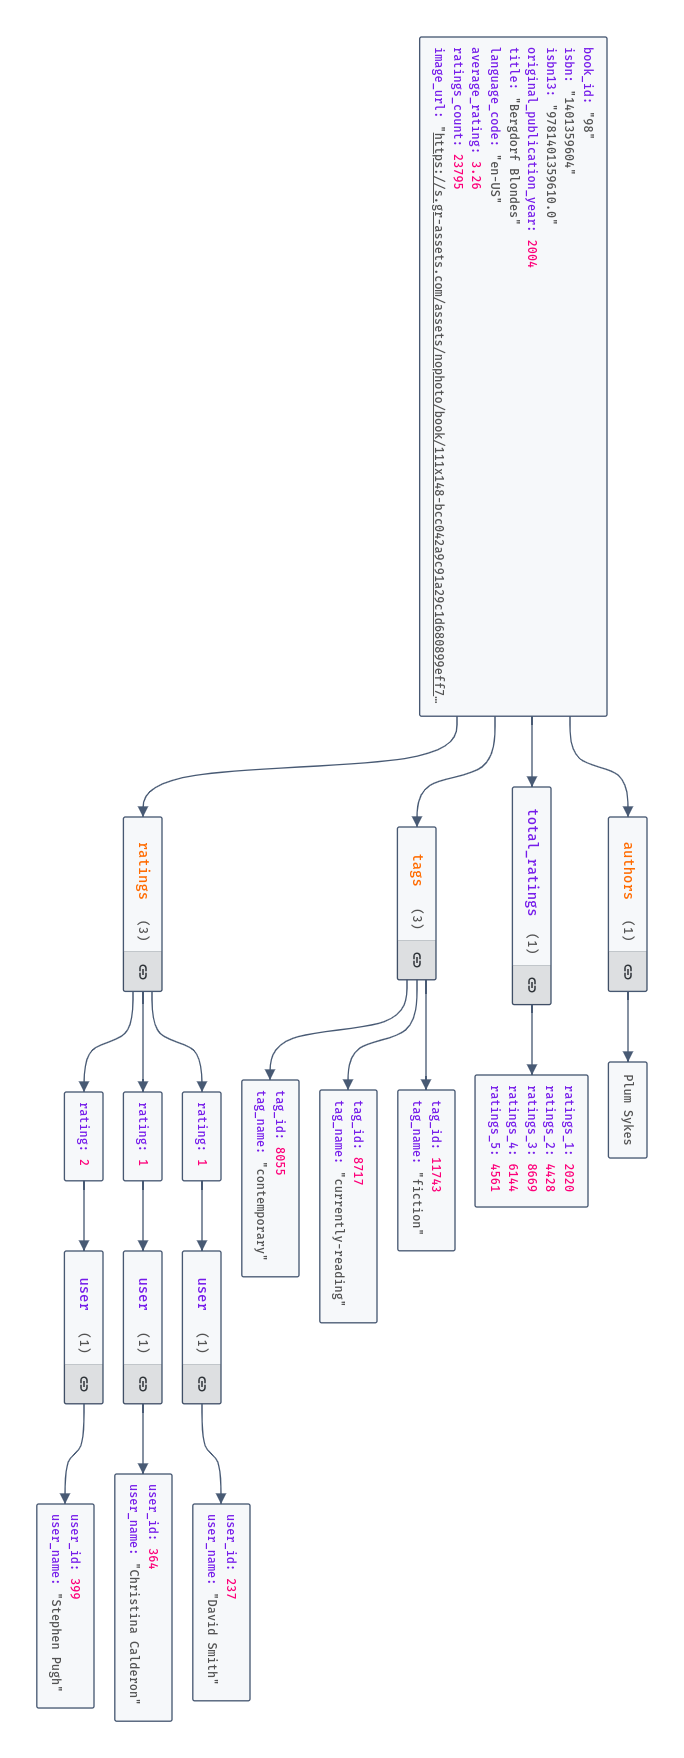
\includegraphics[height=1.2\textwidth]{Collection1Rotate.png}
\end{center}
\restoregeometry
\subsection{Collection 2 - \texttt{users}}
\label{sec:org6b05faa}

\begin{minted}[]{js}
{
    "user_id": 1,
    "user_name": "Mary Martinez",
    "ratings": [
        {
            "book": {
                "book_id": 47,
                "authors": [
                    "Markus Zusak"
                ],
                "title": "The Book Thief",
                "isbn": "375831002",
                "isbn13": 9780375831000.0,
                "language_code": "eng",
                "average_rating": 4.36,
                "ratings_count": 1159741,
                "image_url": "https://images.gr-assets.com/books/1390053681m/19063.jpg",
                "tags": [
                    {
                        "tag_id": 11557,
                        "tag_name": "favorites"
                    },
                    {
                        "tag_id": 30574,
                        "tag_name": "to-read"
                    },
                    {
                        "tag_id": 14487,
                        "tag_name": "historical-fiction"
                    },
                    {
                        "tag_id": 11743,
                        "tag_name": "fiction"
                    },
                    {
                        "tag_id": 33114,
                        "tag_name": "young-adult"
                    }
                ]
            },
            "rating": 3
        }
    ],
    "to_read": [
        {
            "book": {
                "book_id": 112,
                "authors": [
                    "Jojo Moyes"
                ],
                "title": "Me Before You",
                "isbn": "670026603",
                "isbn13": 9780670026610.0,
                "language_code": "eng",
                "average_rating": 4.27,
                "ratings_count": 587647,
                "image_url": "https://images.gr-assets.com/books/1357108762m/15507958.jpg",
                "tags": [
                    {
                        "tag_id": 30574,
                        "tag_name": "to-read"
                    },
                    {
                        "tag_id": 11557,
                        "tag_name": "favorites"
                    },
                    {
                        "tag_id": 17213,
                        "tag_name": "kindle"
                    },
                    {
                        "tag_id": 26138,
                        "tag_name": "romance"
                    },
                    {
                        "tag_id": 3389,
                        "tag_name": "audiobook"
                    }
                ]
            }
        }
    ]
}
\end{minted}

\newgeometry{margin=0in}
\begin{center}
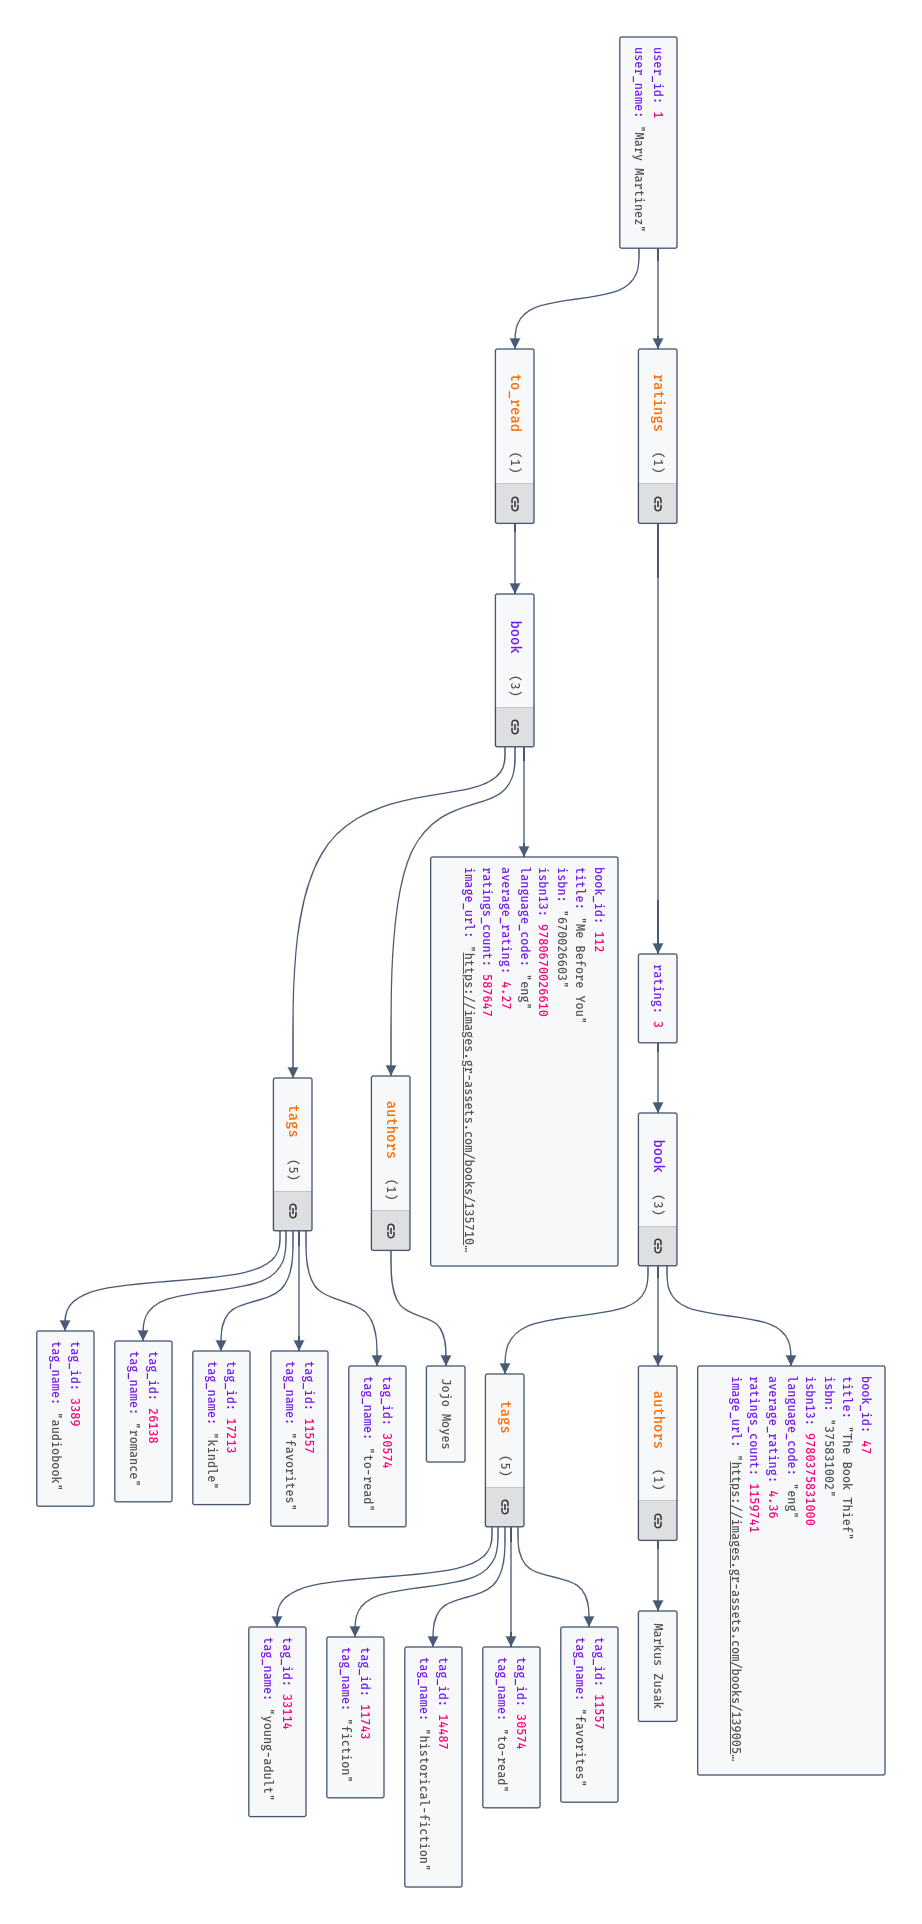
\includegraphics[height=1.2\textwidth]{Collection2Rotate.png}
\end{center}
\restoregeometry
\subsection{Explanation and Justification}
\label{sec:orge040c08}
The data in CSV format emulates the functionality of a relational database. Many of the fields have foreign keys that point to elements in the other CSV files. Document store database favour efficiency over consistency, thus, we have nested a copy of the relevant object where the value would have otherwise been a foreign key. The process by how this was achieved was highlighted in ``\hyperref[sec:org27bc270]{Data Pre-Processing}''.

The data was seeded into the following 2 collections:
\begin{itemize}
\item \texttt{books}
\item \texttt{users}\\
\end{itemize}
\linebreak
\subsubsection{Books}
\label{sec:orga9d0eca}
The \texttt{books} collection roughly followed the format of \texttt{books.csv} (outlined in ``\hyperref[sec:org9be7cf1]{Data Set Explanation}'') with some modifications. We omitted unnecessary information and altered the names of some of the properties to make their semantic meaning clearer. As a result each book document includes:
\begin{itemize}
\item General information about the book (\texttt{title}, \texttt{author}, \texttt{original\_publication\_year}, etc.).
\item Aggregated rating values (\texttt{average\_rating}, \texttt{total\_ratings}, \texttt{ratings\_counts}).
\item A \texttt{ratings} list
\begin{itemize}
\item Each element represents a \texttt{user}'s review of that book. It includes the \texttt{user}'s basic information and the assigned \texttt{rating} score.
\end{itemize}
\item A \texttt{tags} list. Each tag represents a genre or category the book belongs to.\\
\end{itemize}
\linebreak
The most significant element of our design was the aforementioned nesting. Rather than store a separate \texttt{tags} collection, all the tags associated with the book are stored as a list of objects. The same is true for \texttt{ratings}, which is a list of rating objects.\\
\linebreak
Use case examples:\\
\begin{itemize}
\item Collection of books: Querying to see the average rating of a book and the distribution of ratings of a particular book
\end{itemize}
\subsubsection{Users}
\label{sec:orga38b477}
Unlike \texttt{books}, the \texttt{users} collection does not directly correspond to a csv file. Instead, \texttt{users} was created by combining data from \texttt{ratings.csv}, \texttt{to\_read.csv}, and \texttt{books.csv}. We chose to create the user collection in order to demonstrate the importance of collection design with regards to query efficiency. While the \texttt{users} contains a lot of duplicate data from \texttt{books}, it does so in a way that places information about the users at the top of the nesting hierarchy. This means that data about individual users can be obtained without performing expensive joins. The chosen collection design allows one to access, store and perform analytics from the perspective of the user. Each document in the \texttt{users} collection includes the following:
\begin{itemize}
\item A \texttt{user\_id} and \texttt{user\_name} (randomly generated, as explained in ``\hyperref[sec:org27bc270]{Data Pre-Processing}'').
\item A \texttt{ratings} list:
\begin{itemize}
\item Each element represents a score that the user has given to a book.
\item The element includes a \texttt{book} object and a given \texttt{rating} score.
\item The nested \texttt{book} object includes all high-level data about that book, as would be found in the \texttt{books} collection.
\end{itemize}
\item A \texttt{to\_read} list.
\begin{itemize}
\item Each element represents a book that the user has added to their \texttt{to\_read} list (ie. plans to read that book).
\item The element is represented as a \texttt{book} object that is identical in structure to those represented in the \texttt{ratings} list.\\
\end{itemize}
\end{itemize}
\linebreak
Use case examples:\\
        Collection of users: what books user X wants to read.
\section{Create and Load This MongoDB Database}
\label{sec:org596da33}
\subsection{Load the Database}
\label{sec:org80d0c4f}
The process of creating and loading the database was significantly simplified on account of the fact that we had already \hyperref[sec:org27bc270]{Pre-Processed} the data into JSON format. For each collection, a shell command is called to seed the JSON data into their associated collections. The creation of the database is implicit ie. inserting data into the non-existent database leads to its creation. The commands use \texttt{mongoimport}, a CLI tool designed for extracting data from plain-text formats (eg. JSON) and inserting them into MongoDB databases.
\subsubsection{Books Collection}
\label{sec:org6e0d138}
\begin{minted}[]{bash}
mongoimport --db bookstore --collection books --file mongo-seed/books.json --jsonArray
\end{minted}
\subsubsection{Users Collection}
\label{sec:org70a11c5}
\begin{minted}[]{bash}
mongoimport --db bookstore --collection users --file mongo-seed/users.json --jsonArray
\end{minted}
\subsection{Testing}
\label{sec:org0ec13b1}
The shell commands were tested and the output has been annotated on the following page:
\newgeometry{margin=0.1in}
\begin{center}
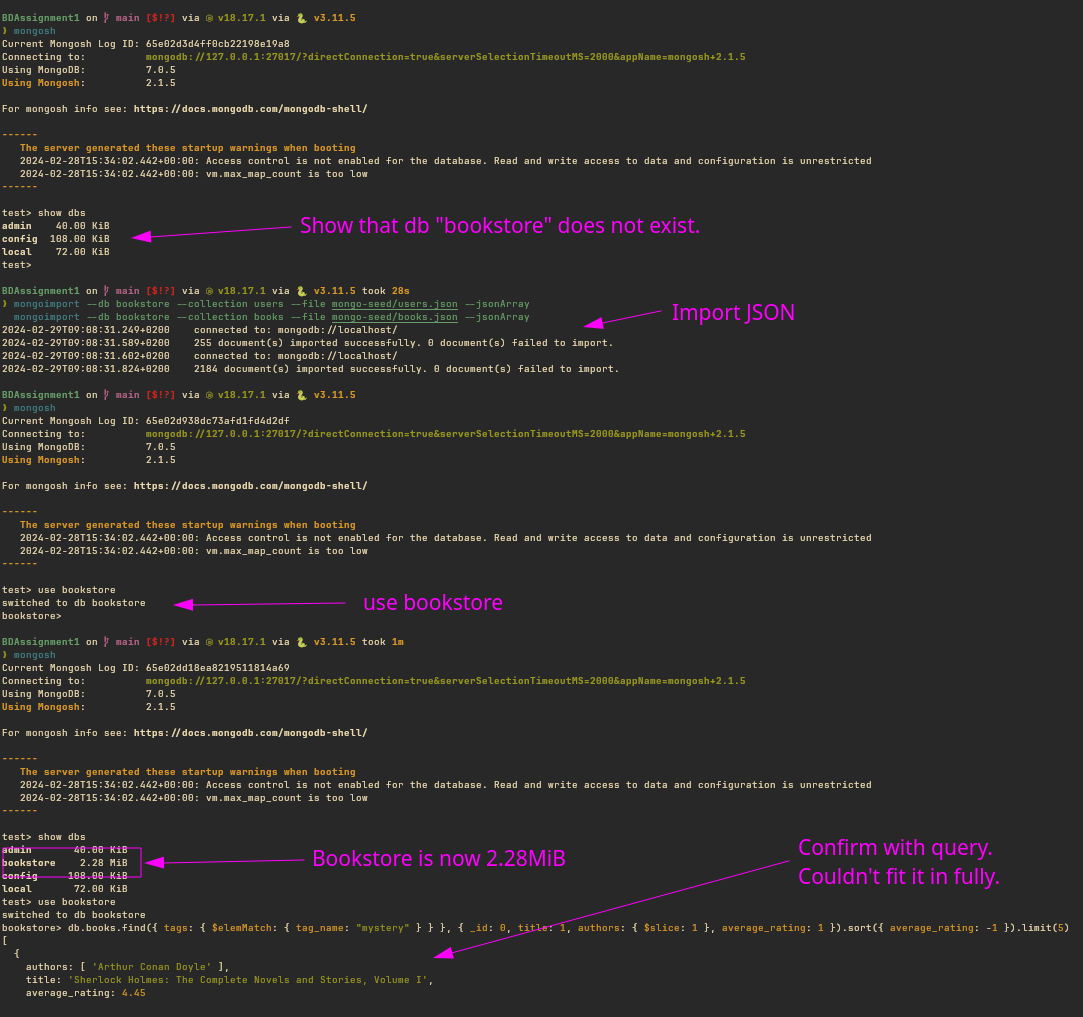
\includegraphics[width=1\textwidth]{q3.png}
\end{center}
\restoregeometry
\section{Discuss the Relative Benefits and Disadvantages of MongoDB}
\label{sec:orgd9a2eb3}
\subsection{MongoDB (Document Store)}
\label{sec:orgfd5269a}
MongoDB is a document store database. Document store databases favour low retrieval latency and efficiency over consistency and functionality (expressiveness) when compared with relational databases. MongoDB is flexible: it fascilitates incremental schema modification as the schema is not rigidly defined. This can improve development velocity and account for changing stakeholder requirements.\\
\linebreak
MongoDB is highly scalable and will be efficient with the ever increasing addition of books being published. MongoDB meets a good middle-ground when compared with other NoSQL databases. It is fascilitates nested data and objects and allows querying on those objects without being overly strict or complex. Each Book and User is able to store all necessary information while allow for performant data retrieval without the overhead of complex joins.\\
\linebreak
The disadvantages of using a MongoDB is that there is a high degree of duplication and redundant data. This means that storing and transferring all of this data is computationally expensive. Secondly, inserting and updating data can be much more expensive than a relational database on account of the necessity to make updates in multiple places (due to the duplication). However, data about books is unlikely to change frequently (as the book has already been published) and thus this downside is heavily mitigated in the chosen example.

\begin{itemize}
\item \textbf{Benefits} (When compared with relational): Scalable, schema-free design, data-access performance
\item \textbf{Disadvantages} (When compared with relational): Duplication, high storage use, slow modification, poor query expressiveness (functionality)
\item \textbf{Role in polyglot persistence}:
\begin{itemize}
\item A future polyglot design could store data that is high in volume but does not change frequently inside a document store db.
\item Books do not change frequently so the information about the books could be stored in the document store while users and ratings could be stored in other databases.
\item User telemetry could also be stored as in a document store database as it is high volume with very infrequent modification
\end{itemize}
\end{itemize}
\subsection{Graph DB}
\label{sec:org858c0ca}
Graph based databases allow for expressive and performant relationship representation and would be ideal for relationship related queries. Each relationship can be given properties that qualitatively describe that relationship. This is ideal for data where the relationships to other data is the primary provider of utility (eg. a knowledge graph), as opposed to the structured categorisation (as is the case in MongoDB and relational databases).\\
\linebreak
The chosen dataset is highly structured without a large number of annotated relationships between data and it thus be a poor choice for graph DBs. The dataset would not leverage the benefits of a graph DB and would miss out on the well-fitted the benefits of MongoDB, namely schema flexibility, performance, and scalability, and simplicity.

\begin{itemize}
\item \textbf{Benefits}: Efficient modelling of highly inter-linked data, Query expressiveness (functionality), Great relationship representation (for which it is scalable and performant)
\item \textbf{Disadvantages}: Unnecessary complexity, poor modelling of structured data
\item \textbf{Role in polyglot persistence}:
\begin{itemize}
\item A future polyglot design could include a graph database that models the relationship books have to each other.
\item Each book could have an outgoing edge to related books with a descriptive tag that describes their relationship strength and type.
\item This would prove highly useful for the sites recommendation engine.
\end{itemize}
\end{itemize}
\subsection{Key-value Store}
\label{sec:org8312570}
Key-Value stores are extremely simple. They very similar to a document store but with fewer cabilities in data representation and querying. They offer many of the same benefits of schema flexibility, scalability, and performance. There key benefit and disadvantage over document stores is their simplicity. The simplicity is limiting but ideal for data that can be modelled simply. The chosen dataset is not suited for a key-value store as it includes more complex nested objects.
\begin{itemize}
\item \textbf{Benefits}: High performance, Scalability, Simplicity, Flexibility
\item \textbf{Disadvantages}: Limited query capabilities and Does not support complex data structures.
\item \textbf{Role in polyglot persistence}:
\begin{itemize}
\item It can store the current session data of users. Easy to keep track of users' sessions such as how long they were on the app.
\item The key-value store's flexability would be very important as it would allow us to store more complex session information about the user which can be used for processing later on to improve the users experience on the application.
\end{itemize}
\end{itemize}
\subsection{Relational}
\label{sec:org1f19c44}
Relational databases are great for keeping data consistent and for effectively maintaining the relationships of the data. Their ability to store relationships (via foreign keys) between data ensures the following benefits: data consistency, minimal duplication, expressive queries. Relational databases falter when needing to retrieve large quantities of data from different tables. Joins become very expensive as the size of a dataset grows. Data analysis and operations are impacted substantially. It becomes inefficient with a very large (big) data.\\
\linebreak
The goodbooks dataset at present would be well suited to a relational database, however, if we were to massively increase the scale of the data stored the efficiency gains of MongoDB would quickly become apparent. The data is not updated frequently enough and for critical operations and thus the consistency benefits provided by a relational database would be negligible.

\begin{itemize}
\item \textbf{Benefits}: Query Expressiveness (functionality), consistency, reliability, low storage use (avoids duplication), accuracy, data integrity
\item \textbf{Disadvantages}: Decrease in performance at scale, low flexibility (requires up-front schema design)
\item \textbf{Role in polyglot persistence}:
\begin{itemize}
\item A future polyglot design could include a relational database for data that would benefit from reliability and consistency.
\item Information about users, including their profiles, and security information could be stored in this format.
\item User data could benefit from the expressive queries provided by relational databases.
\end{itemize}
\end{itemize}
\subsection{Column Family}
\label{sec:org2fc21ef}
Column Family DBs are similar to relational databases, however, they bundle groups of frequently accessed columns together. This reduces the performance issues that may occur in relational databases. It does, however, still require up-front schema design without obtaining the expressiveness benefits provided by relational databases.\\
\linebreak

At present, the good reads database are not well suited to being effectively grouped. The only instance in which this would be useful would be a bundling of ratings data in the books table. However, the benefits are not extensive enough to utilise this over MongoDB for this dataset.

\begin{itemize}
\item \textbf{Benefits}: Compression of data, Scalable, fast to load queries, good for simple analytics.
\item \textbf{Disadvantages}: Limited querying capabilities, limited data modelling capabilities
\item \textbf{Role in polyglot persistence}:
\begin{itemize}
\item A future polyglot design could include a column family for calculating metrics and performance analytics, such as:
\begin{itemize}
\item How many books are users reading and the total number of stars people rated individual books
\item How long people stay on the website, etc.
\end{itemize}
\item Each set of metrics relating to a particular type of user data could be grouped into a column family for that user.
\end{itemize}
\end{itemize}
\subsection{Hierarchical}
\label{sec:orgf2a1eba}
Hierarchical databases are optimised for data that can be stored as deeply nested hierarchies. Document Store DBs are also well suited for hierarchical nesting, however, they access performance greatly suffers when the depth of those hierarchies becomes excessive. Thus, hierarchical databases are great for data with inherently deep hierarchical structure. Hierarchical databases would be effective for fast lookup and to effectively store this data.\\
\linebreak
While the goodbooks dataset does include hierarchies, the hierarchies seldom extend beyond a depth of 5. This means the data is not inherently hierarchical and does not suffer from performance detriments when traversing the nested data. On account of this, a hierarchical database would be a poor choice as it would miss out on the key benefits of MongoDB (flexibility in particular).

\begin{itemize}
\item \textbf{Benefits}: Fast retrieval of nested data, efficient storage of data, predictable data structure
\item \textbf{Disadvantages}: Limited flexibility, hard to maintain and update, limited interoperability, reduced expresiveness
\item \textbf{Role in polyglot persistence}:
\begin{itemize}
\item In the future, the platform may wish to hold a representation of books, their predecessors, and their successors.
\item A hierarchical relationship could be modelled such that each book belongs to a subgenre, which belongs to a series of parent genres. These books would have parent and descendant books that are influenced by them.
\item This hierarchy could be stored separately to the primary book database to avoid affecting its performance and size.
\end{itemize}
\end{itemize}
\section{Query and Updating the Database}
\label{sec:org232269e}
\subsection{GRDDAN017}
\label{sec:orgc1b95f3}
\subsubsection{1}
\label{sec:orgbd74ce5}
\textbf{Description}\\
Find the book title and author list of the top 3 highest rated books.\\
\linebreak
\textbf{Query}
\begin{minted}[]{js}
db.books.find({},{
    _id: false, book_id: true, title: true, authors: true, average_rating: true
}).sort({average_rating:-1}).limit(3);
\end{minted}
\linebreak
\textbf{Output}\\
\begin{center}
\includegraphics[width=1\textwidth]{images/GRDDAN017/1.png}
\end{center}
\pagebreak
\subsubsection{2}
\label{sec:orgc1e7436}
\textbf{Description}\\
Find 2 books with the ``fantasy'' tag with a high average rating.\\
\linebreak
\textbf{Query}
\begin{minted}[]{js}
db.books.find({
    $and: [{ "tags.tag_name": "fantasy" }, { "average_rating": { $gt: 4 } }]
}).limit(2)
\end{minted}
\linebreak
\textbf{Output}\\
\begin{center}
\includegraphics[width=1\textwidth]{images/GRDDAN017/2.png}
\end{center}
\pagebreak
\subsubsection{3}
\label{sec:org3e5c892}
\textbf{Description}\\
Find users who have rated a book but have an empty to\textsubscript{read} list.\\
\linebreak
\textbf{Query}
\begin{minted}[]{js}
db.users.find({
    ratings: { $exists: true, $not: {$size: 0} },
    to_read: { $size: 0 }
}, {
    _id: false, ratings: false
});
\end{minted}
\linebreak
\textbf{Output}\\
\begin{center}
\includegraphics[width=1\textwidth]{images/GRDDAN017/3.png}
\end{center}
\pagebreak
\subsubsection{4}
\label{sec:org70c465a}
\textbf{Description}\\
Add a book to a user's to-read list.\\
\linebreak
\textbf{Query}
\begin{minted}[]{js}
db.users.updateOne({
    "user_id"   : 4
}, {
    $push: {
        "to_read": {
            book: { book_id: 0, authors: ["Daniel Gordon"], title: My Story,
                    isbn: "0", isbn13: 0, average_rating: -1, tags: ["trash"]}
        }
    }
})
\end{minted}

\linebreak
\textbf{Output}\\
\begin{center}
\includegraphics[width=1\textwidth]{images/GRDDAN017/4.png}
\end{center}
\pagebreak
\subsection{MRCGAB004}
\label{sec:org50c69db}
\subsubsection{1}
\label{sec:orgb044275}
\textbf{Description}\\
Find and return a list of users’ names  who want to read “The book Thief”.\\
\linebreak
\textbf{Query}
\begin{minted}[]{js}
db.users.find( {
    "to_read.book.title":"The Book Thief"
}, {
    "_id":0,"user_name":1
})
\end{minted}
\linebreak
\textbf{Output}\\
\begin{center}
\includegraphics[width=1\textwidth]{images/MRCGAB004/1.png}
\end{center}
\pagebreak
\subsubsection{2}
\label{sec:orga479bc0}
\textbf{Description}\\
Find a list of books published after 2004 and return the title and year it was published.\\
\linebreak
\textbf{Query}
\begin{minted}[]{js}
db.books.find({
    "original_publication_year":{ "$gt": 2004 }
},{
    "title":1, "_id":0,"original_publication_year":1
})
\end{minted}
\linebreak
\textbf{Output}\\
\begin{center}
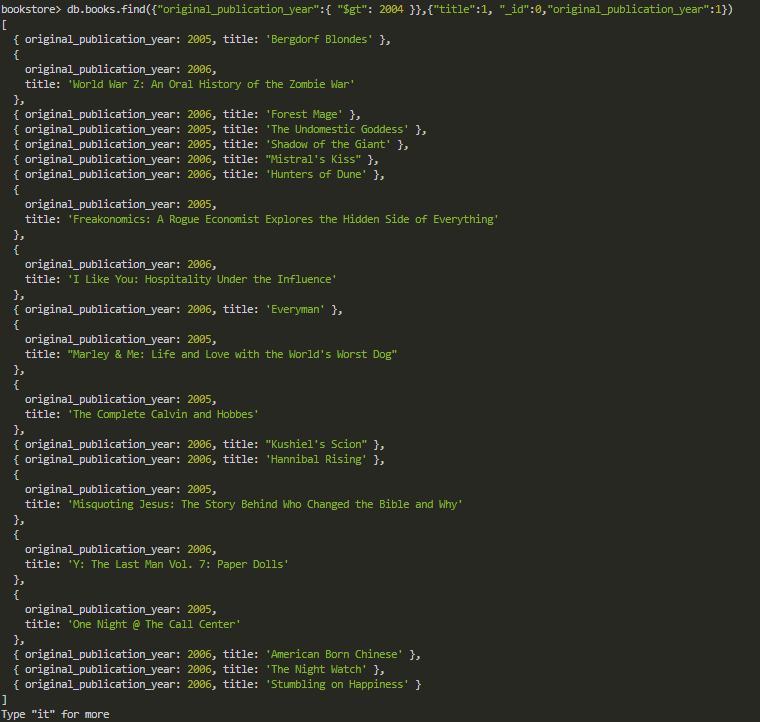
\includegraphics[width=1\textwidth]{images/MRCGAB004/2.png}
\end{center}
\pagebreak
\subsubsection{3}
\label{sec:org14e6c68}
\textbf{Description}\\
Update the book “Bergdorf Blondes” with a new publishing date of 2005 db.books.updateOne. \\
\linebreak
\textbf{Query}
\begin{minted}[]{js}
db.books.updateOne({
    "title":"Bergdorf Blondes"
},{
    "$set":{"original_publication_year":2005}
})
\end{minted}

\linebreak
\textbf{Output}\\
\begin{center}
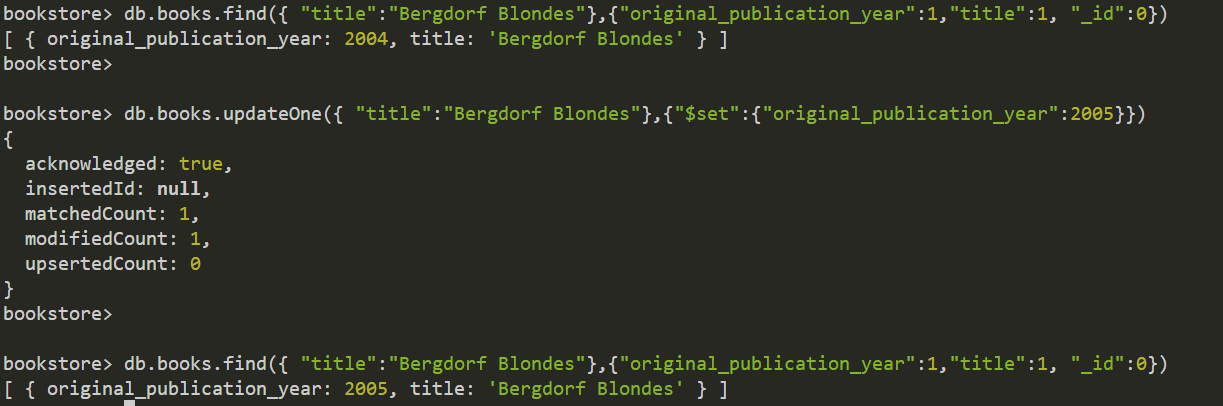
\includegraphics[width=1\textwidth]{images/MRCGAB004/3.png}
\end{center}
\pagebreak
\subsubsection{4}
\label{sec:orgc83ec7a}
\textbf{Description}\\
Delete user with the user\textsubscript{id} 32.\\
\linebreak
\textbf{Query}
\begin{minted}[]{js}
db.users.deleteOne({"user_id":32})
\end{minted}

\linebreak
\textbf{Output}\\
\begin{center}
\includegraphics[width=1\textwidth]{images/MRCGAB004/4.png}
\end{center}
\pagebreak
\subsection{CRGMAT002}
\label{sec:orga9215e1}
\subsubsection{1}
\label{sec:org3fa142e}
\textbf{Description}\\
Find the top 5 books (by average\textsubscript{rating}) with tag\textsubscript{name} ``sci-fi''. Show only a single author for each book. \\
\linebreak
\textbf{Query}
\begin{minted}[]{js}
db.books.find({
    tags: {$elemMatch: {tag_name: "sci-fi"}}
}, {
    _id: 0, title: 1, authors: {$slice: 1}, average_rating: 1,
}).sort({average_rating : -1 }).limit(5)
\end{minted}
\linebreak
\textbf{Output}\\
\begin{center}
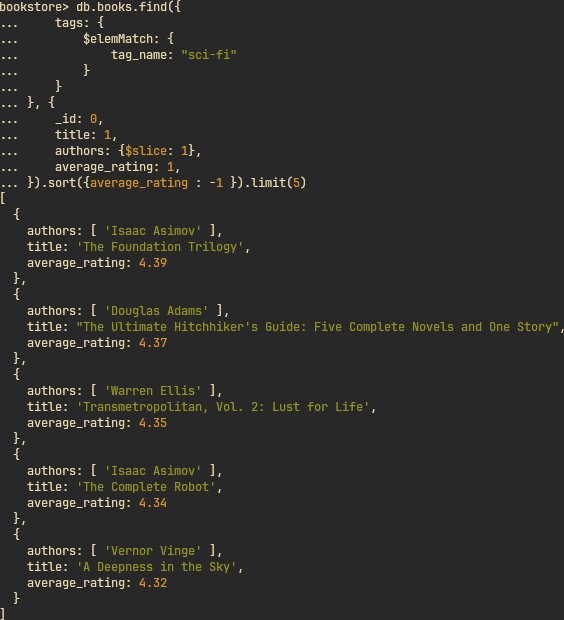
\includegraphics[width=1\textwidth]{images/CRGMAT002/1.png}
\end{center}
\pagebreak
\subsubsection{2}
\label{sec:org12aa113}
\textbf{Description}\\
Aggregate user\textsubscript{ids} alongside the total number of ratings that user has submitted (size of ratings array). The result is sorted by the number of ratings they have submitted and the top 10 are shown. \\
\linebreak
\textbf{Query}
\begin{minted}[]{js}
db.users.aggregate([ {
    $project: {_id: 0, user_id: 1, numRatings: { $size: "$ratings" }}
}, {
    $sort: { numRatings: -1 }
}, {
    $limit: 10
}])
\end{minted}
\linebreak
\textbf{Output}\\
\begin{center}
\includegraphics[width=1\textwidth]{images/CRGMAT002/2.png}
\end{center}
\pagebreak
\subsubsection{3}
\label{sec:org04b9cbf}
\textbf{Description}\\
Update a user that has rated ``The Book Thief'' with 4 stars. Change their name to: ``Update\textsubscript{User}!''\\
\linebreak
\textbf{Query}
\begin{minted}[]{js}
db.users.updateOne({
    "ratings": {$elemMatch: {rating: 4, "book.title": "The Book Thief"}}
},{
    $set: {user_name: "Update_Username!"}
})
\end{minted}
\linebreak
\textbf{Output}\\
\begin{center}
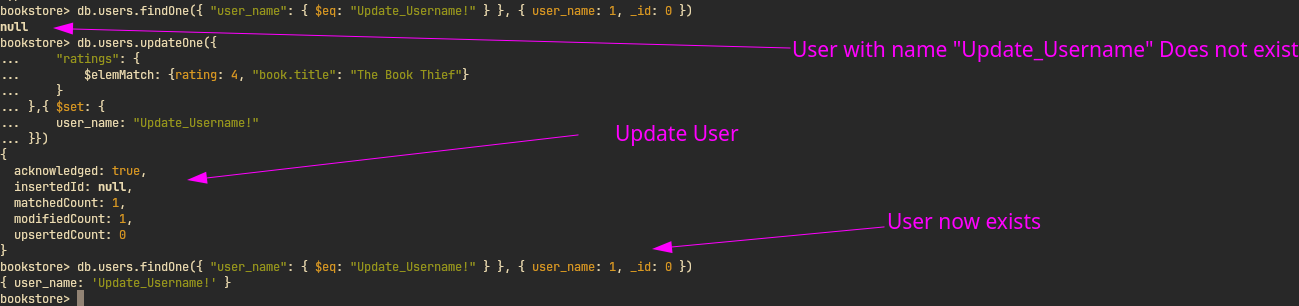
\includegraphics[width=1\textwidth]{images/CRGMAT002/3.png}
\end{center}
\pagebreak
\subsubsection{4}
\label{sec:org4f10494}
\textbf{Description}\\
test\\
\linebreak
\textbf{Query}
\begin{minted}[]{js}
db.books.deleteMany({
    authors: "Roald Dahl"
},{
    title: 1
})
\end{minted}

\linebreak
\textbf{Output}\\
\begin{center}
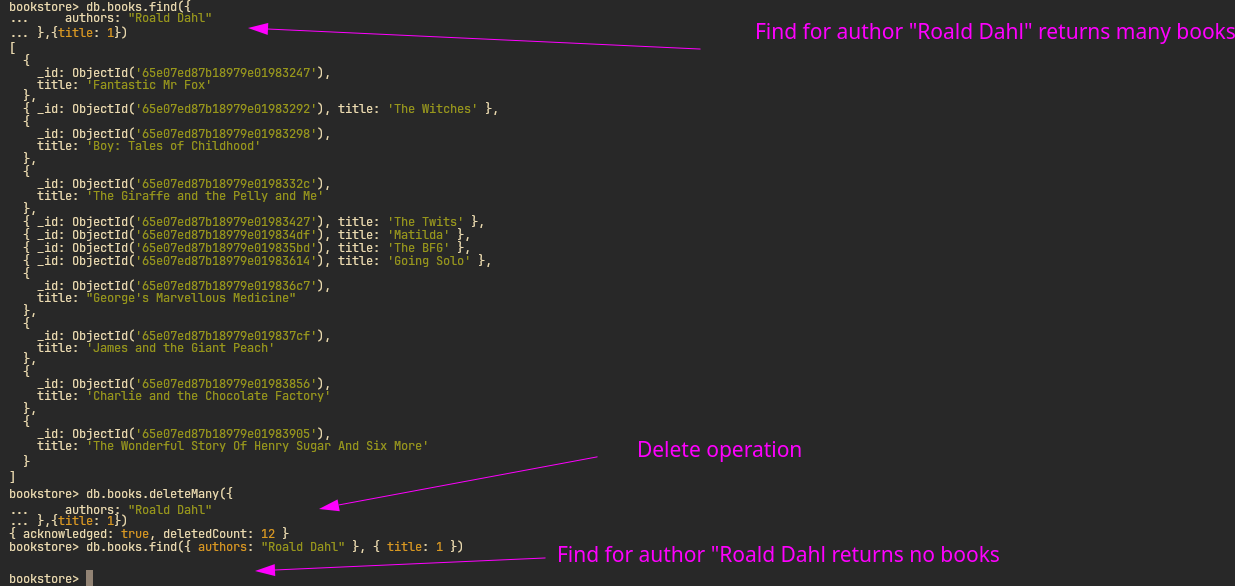
\includegraphics[width=1\textwidth]{images/CRGMAT002/4.png}
\end{center}
\pagebreak
\subsection{WHLJOS001}
\label{sec:org0135db8}
\subsubsection{1}
\label{sec:org41186bf}
\textbf{Description}\\
Find the names and ratings of the top 50 fiction books with at least 1000 ratings.\\
\linebreak
\textbf{Query}
\begin{minted}[]{js}
db.books.aggregate([{
    $match: { "total_ratings": { $gte: 1000 }, "tags.tag_name": "fiction" }
}, {
    $sort: { "average_rating": -1 }
}, {
    $limit: 50
}, {
    $project: { _id: 0, title: 1, average_rating: 1 }
}] )
\end{minted}
\linebreak
\textbf{Output}\\
\begin{center}
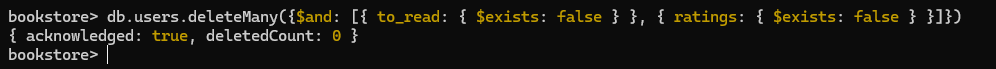
\includegraphics[width=1\textwidth]{images/WHLJOS001/1.png}
\end{center}
\pagebreak
\subsubsection{2}
\label{sec:org96b8b33}
\textbf{Description}\\
Delete all users who have never rated a book and never marked a book as to\textsubscript{read}:

\linebreak
\textbf{Query}
\begin{minted}[]{js}
db.users.deleteMany({
    $and: [{to_read: { $exists: false }},
           {ratings: { $exists: false }}]
})
\end{minted}

\linebreak
\textbf{Output}\\
\begin{center}
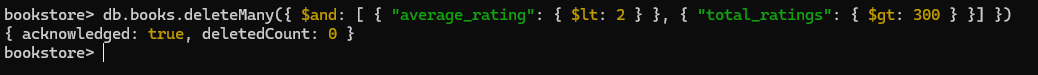
\includegraphics[width=1\textwidth]{images/WHLJOS001/2.png}
\end{center}
\pagebreak
\subsubsection{3}
\label{sec:org320afee}
\textbf{Description}\\
Delete all books with an average rating less than 2 and more than 300 ratings.\\
\linebreak
\textbf{Query}
\begin{minted}[]{js}
db.books.deleteMany({
    $and: [ {
        "average_rating": { $lt: 2 }
    }, {
        "total_ratings": { $gt: 300 }
    }]
})
\end{minted}
\linebreak
\textbf{Output}\\

\begin{center}
\includegraphics[width=1\textwidth]{images/WHLJOS001/3.png}
\end{center}
\pagebreak
\subsubsection{4}
\label{sec:org27a5479}
\textbf{Description}\\
Find the name of the user who has rated the most books.\\
\linebreak
\textbf{Query}
\begin{minted}[]{js}
db.users.aggregate({
    $project: { user_id: 1, user_name: 1, num_ratings: { $size: "$ratings" } }
},{
    $sort: { num_ratings: -1 }
},{
    $limit: 1
}, {
    $project: {
        _id: 0, user_name: 1
    }
})
\end{minted}

\linebreak
\textbf{Output}\\
\begin{center}
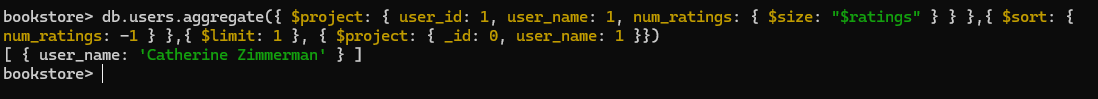
\includegraphics[width=1\textwidth]{images/WHLJOS001/4.png}
\end{center}
\section{Link the Database to a Program}
\label{sec:org2aada2e}

\section{Contribution Statement}
\label{sec:org657dedd}
\begin{center}
\begin{tabular}{ll}
\hline
Task & Who did it\\
Design Schema/JSON & Matthew \& Gabe\\
Setup Devops (Github, Docker) & Jordy\\
Preprocessing & Joe \& Daniel\\
Create the App & Jordy\\
Query & Everyone\\
Load into mongodb & Mathew\\
Write Up & Gabe \& Matthew \& Daniel\\
\hline
\end{tabular}
\end{center}
\end{document}
